\documentclass[12pt, a4paper]{article}
\usepackage[LGR, T1]{fontenc}
\usepackage[utf8]{inputenc}
\usepackage[greek]{babel}
\usepackage{cite}
\usepackage{hyperref}
\usepackage{xcolor}
\usepackage[ruled, linesnumbered]{algorithm2e}
\usepackage[document]{ragged2e}
\usepackage{graphicx}
\usepackage{float}
\graphicspath{ {./images/} }

\setlength{\parindent}{0em}

\title{{ΗΥ3604 Ενσωματωμένα Συστήματα Πραγματικού Χρόνου}\newline
{\large Αριστοτέλειο Πανεπιστήμιο Θεσσαλονίκης}\newline
{Εργασία 1\textsuperscript{η}}}
\author{Δημήτριος Αντωνιάδης\\
8462
\\\textlatin{akdimitri@auth.gr}}
\date{Μάιος 2019}

\begin{document}
\maketitle
\pagebreak
\tableofcontents
\pagebreak
%1ο κεφάλαιο Εισαγωγή
%   1η Εισαγωγική Παράγραφος
\section{Εισαγωγή.}
\justify
Το παρόν έγγραφο αποτελεί την αναφορά της πρώτης (1\textsuperscript{ης}) εργασίας που πραγματοποιήθηκε στο πλαίσιο του μαθήματος \textit{"Ενσωματωμένα Συστήματα Πραγματικού Χρόνου"}. Σκοπός της εργασίας είναι να γίνει τακτική δειγματοληψία με την μικρότερη δυνατή απόκλιση από τον
πραγματικό χρόνο. Στο πείραμα αυτό οι τιμές της δειγματοληψίας είναι τα \textlatin{\textbf{timestamps}} που επιστρέφει η συνάρτηση \textlatin{\textbf{gettimeofday()}}\cite{manual}.

%2η παράγραφος Δομή της εργασίας
\justify
Παραπάνω παρουσιάστηκε μία σύντομη εισαγωγή αναφορικά με το θέμα της παρούσας αναφοράς. Στη δεύτερη (2\textsuperscript{η}) ενότητα παρουσιάζονται τα αρχεία που περιλαμβάνει η εργασία αυτή και η μέθοδος του \textit{\textlatin{Compilation}}. Στην τρίτη (3\textsuperscript{η}) ενότητα παρουσιάζονται οι δύο αλγόριθμοι που υλοποιήθηκαν και στην τέταρτη (4\textsuperscript{η}) ενότητα τα αποτελέσματα τους. Τέλος, στην πέμπτη (5\textsuperscript{η}) παρουσιάζονται τα συμπεράσματα της εργασίας αυτής.


%2ο Κεφάλαιο Περιεχόμενα Φακέλου Εργασίας και Μέθοδος Compilation
\section{Φάκελος υποβολής, \textlatin{Compilation} και Εκτέλεση.}
Ο φάκελος υποβολής με τον πηγαίο κώδικα βρίσκεται στην παρακάτω διεύθυνση:
%URL Github
\begin{itemize}
  \item \textlatin{\color{blue}{\url{https://github.com/akdimitri/RTES1}}}
\end{itemize}
Στον φάκελο \textit{\textlatin{code}} περιλαμβάνονται δύο (2) αρχεία. Τα αρχεία:
%Περιεχομενα ./code
\begin{itemize}
  \item \textlatin{simple.c}
  \item \textlatin{advanced.c}
\end{itemize}
\justify
Το πρώτο αρχείο αποτελεί το ζητούμενο πηγαίο κώδικα της εργασίας ο οποίος δεν κάνει χρήση των προηγούμενων
\textit{\textlatin{timestamps}}. Το δεύτερο αρχείο αποτελεί το ζητούμενο πηγαίο κώδικα της εργασίας ο οποίος κάνει χρήση των προηγούμενων \textit{\textlatin{timestamps}} με σκοπό την ακριβή δειγματοληψία πραγματικού χρόνου.
\justify
Το \textit{\textlatin{Compilation}} των δύο παραπάνω αρχείων πραγματοποιείται με τις εξής εντολές:
%Compilation
\begin{itemize}
  \item \textlatin{gcc simple.c -o simple -O3}
  \item \textlatin{gcc advanced.c -o advanced -O3}
\end{itemize}

%Execution
\justify
Η εκτέλεση και των δύο εκτελέσιμων αρχείων πραγματοποιείται με τον ίδιο τρόπο. Η εκτέλεση απαιτεί δύο ορίσματα. Το πρώτο όρισμα αντιπροσωπεύει το χρόνο εκτέλεσης του πειράματος σε \textbf{ώρες} και το δεύτερο όρισμα το χρονικό διάστημα που μεσολαβεί μεταξύ δύο δειγματοληψιών σε \textbf{δευτερόλεπτα}. Για παράδειγμα, με τις παρακάτω εντολές εκτελούνται τα πειράματα για 2 ώρες με χρονικό διάστημα μεταξύ δύο \textlatin{timestamps} ίσο με 0.1 δευτερόλεπτα:
\begin{itemize}
  \item \textlatin{./simple 2 0.1}
  \item \textlatin{./advanced 2 0.1}
\end{itemize}

%Rstudio
\justify
Επιπλέον, στο \textlatin{repository} περιλαμβάνεται ο φάκελος \textit{\textlatin{Rstudio}} ο οποίος περιέχει το αρχείο \textlatin{\textbf{script.r}} με το οποίο γίνεται η ανάλυση των αποτελεσμάτων και εξάγονται τα διαγράμματα. Ακόμη, περιλαμβάνεται και το αρχείο \textlatin{\textbf{regex.R}}, το οποίο χρησιμοποιείται για την μελέτη της υπολογιστικής ισχύς του προγράμματος.

%Resutls
\justify
Τέλος, περιλαμβάνεται στο repository και ένας φάκελος με ενδεικτικές μετρήσεις.

\section{Αλγόριθμοι.}
Στην παρούσα ενότητα παρουσιάζονται οι δύο αλγόριθμοι που πραγματοποιήθηκαν σε μορφή ψευδογλώσσας ώστε να είναι εύκολα κατανοητοί.

\subsection{Αλγόριθμος \textlatin{simple}}
Στην υποενότητα αυτή παρουσιάζεται ο αλγόριθμος που υλοποιείται από τον πηγαίο κώδικα \textlatin{\textit{simple.c}}. Το πρόγραμμα δέχεται ως όρισμα το συνολικό χρόνο εκτέλεσης του προγράμματος (\textlatin{\textit{executionTime}}) και το διάστημα (\textlatin{\textit{interval}}) που μεσολαβεί μεταξύ δύο δειγματοληψιών χρόνου. Συνεπώς, είναι δυνατό διαιρώντας το συνολικό χρόνο εκτέλεσης με το χρονικό διάστημα μεσολάβησης να βρεθεί ο συνολικός αριθμός χρονικών διαστημάτων μεσολάβησης μεταξύ των δειγματοληψιών. Για να πραγματοποιηθούν τόσα διαστήματα μεσολάβησης απαιτείται να ληφθούν ισόποσα στιγμιότυπα χρόνου (\textlatin{\textit{timestamps}}) συν ένα (1) επιπλέον. Η μεταβλητή που αναπαριστά τον αριθμό των συνολικών στιγμιοτύπων που θα ληφθούν ονομάζεται \textlatin{\textit{iterations}}.
\justify
Η δειγματοληψία των χρονικών στιγμών πραγματοποιείται με τη χρήση της συνάρτησης
\begin{itemize}
\item \textlatin{\textit{gettimeofday(struct timeval *tv,
    struct timezone *tz)}}\cite{manual}
\end{itemize}
η οποία επιστρέφει σε κατάλληλη δομή (\textlatin{struct}) το χρόνο που έχει παρέλθει από τη χρονική στιγμή \textlatin{\textit{Epoch}}, δηλαδή τη χρονική στιγμή 1970-01-01 00:00:00 +0000 (\textlatin{UTC}).
\justify
Το διάστημα που μεσολαβεί μεταξύ της δειγματοληψίας δύο χρονικών στιγμών πραγματοποιείται με τη χρήση της συνάρτησης
\begin{itemize}
    \item \textlatin{\textit{usleep( useconds\_t usec)}}\cite{manual}
\end{itemize}
Η συνάρτηση αυτή αναστέλλει την εκτέλεση του \textlatin{thread} που εκτελείται για χρονικό διάστημα \textlatin{\textit{usec}}.
\newline
\justify
\textlatin{
\begin{algorithm}[H]
\SetKwData{Left}{left}\SetKwData{This}{this}\SetKwData{Up}{up}
\SetKwFunction{Union}{Union}\SetKwFunction{FindCompress}{FindCompress}
\SetKwInOut{Input}{input}\SetKwInOut{Output}{output}
\Input{$executionTime(HOURS), interval(SECONDS)$}
\Output{$timestamps$ MATRIX[$iterations$, 1] }
 $iterations \longleftarrow (executionTime)*3600/interval + 1$
 \BlankLine
 \BlankLine
 $timestamps[1] \longleftarrow gettimeofday(...)$\\
 \For{$i \leftarrow 2$ : $iterations$}{
  usleep($interval*1000000$)\\
  $timestamps[i] \longleftarrow gettimeofday(...)$
 }
 export $timestamps$ MATRIX to a text file
 \caption{simple.c}
\end{algorithm}}


\subsection{Αλγόριθμος \textlatin{advanced}.}
Ο αλγόριθμος αυτός δειγματοληπτεί τόσες χρονικές στιγμές όσες και ο παραπάνω. Η μόνη διαφορά είναι ότι ο παραπάνω αλγόριθμος αποτυγχάνει τα δειγματοληπτήσει με την ακρίβεια που δειγματοληπτεί ο \textlatin{advanced}. Ο αλγόριθμος που παρατίθεται παρακάτω κάνει χρήση των προηγούμενων χρονικών στιγμών που έχουν ληφθεί κατά τη δειγματοληψία ώστε να βελτιώσει την απόδοση του. Συγκεκριμένα, εφόσον είναι γνωστή η πρώτη τιμή δειγματοληψίας και το χρονικό διάστημα που μεσολαβεί μεταξύ δύο δειγματοληψιών είναι δυνατό να γνωρίζουμε και την ακριβή στιγμή που πρέπει να πραγματοποιηθεί η δειγματοληψία της τιμής $i$. Δηλαδή,\newline 

\centering{$timestamps[i] \longleftarrow timestamps[1] + i*interval$}

\justifyΕπομένως, για κάθε τιμή δειγματοληψίας είναι γνωστή και η αναμενόμενη τιμή της. Έτσι, για κάθε τιμή δειγματοληψίας μπορεί να υπολογιστεί και η χρονική απόκλιση και να αφαιρεθεί από το επόμενο χρονικό διάστημα μεσολάβησης.
\newline

\justify
\textlatin{
\begin{algorithm}[H]
\SetKwData{Left}{left}\SetKwData{This}{this}\SetKwData{Up}{up}
\SetKwFunction{Union}{Union}\SetKwFunction{FindCompress}{FindCompress}
\SetKwInOut{Input}{input}\SetKwInOut{Output}{output}
\Input{$executionTime(HOURS), interval(SECONDS)$}
\Output{$timestamps$ MATRIX[$iterations$, 1] }
 $iterations \longleftarrow (executionTime)*3600/interval + 1$\\
 $delay \longleftarrow 0$
 \BlankLine
 \BlankLine
 $timestamps[1] \longleftarrow gettimeofday(...)$\\
 \For{$i \leftarrow 2$ : $iterations$}{
  usleep($interval*1000000 - delay$)\\
  $timestamps[i] \longleftarrow gettimeofday(...)$
  $delay \longleftarrow timestamps[i] - i*interval - timestamps[0]$
 }
 export $timestamps$ MATRIX to a text file
 \caption{advanced.c}
\end{algorithm}}

%4η Ενοτητα Αποτελέσματα Πειραματων.
\section{Αποτελέσματα.}
\justify
Στην ενότητα αυτή παρουσιάζονται τα αποτελέσματα από την εκτέλεση των παραπάνω αλγορίθμων. Τα παρακάτω διαγράμματα προκύπτουν ύστερα από την επεξεργασία των δεδομένων μέσω του προγράμματος \textlatin{\textbf{\textit{Rstudio}}}. Το \textlatin{\textit{script.r}} περιλαμβάνει όλες τις εντολές για την εξαγωγή των παρακάτω αποτελεσμάτων και διαγραμμάτων.

\subsection{Αποτελέσματα αλγορίθμου \textlatin{simple}.}
\justify
Η εκτέλεση του αλγορίθμου αυτού με ορίσματα:
\begin{itemize}
    \item $executionTime \longleftarrow 2$
    \item $interval \longleftarrow 0.1$
\end{itemize}
είχε συνολικό χρόνο: $7207.682$ $secs$ δηλαδή καθυστέρησε για περίπου \textbf{7.5} δευτερόλεπτα. Η μέση τιμή ήταν \textbf{100106.7 \textlatin{usec}}, δηλαδή μεταξύ κάθε κάθε μέτρησης υπήρχε καθυστέρηση περίπου 107 μικρο-δευτερολέπτων. Η τυπική απόκλιση ήταν \textbf{18.024}.

\justify
Οπως φαίνεται και από τα παρακάτω διαγράμματα στο σύνολό τους οι τιμές ήταν μεγαλύτερες των 100000 \textlatin{usec} που ήταν η επιθυμητή τιμή, για το λόγο αυτό παρατηρήθηκε και αυτή η απόκλιση. 
\begin{figure}[H]
        
        \caption{\centering{Τιμές διαστημάτων μεσολάβησης μεταξύ 2 δειγματοληψιών του αλγορίθμου \textlatin{simple}}}
        \centering
        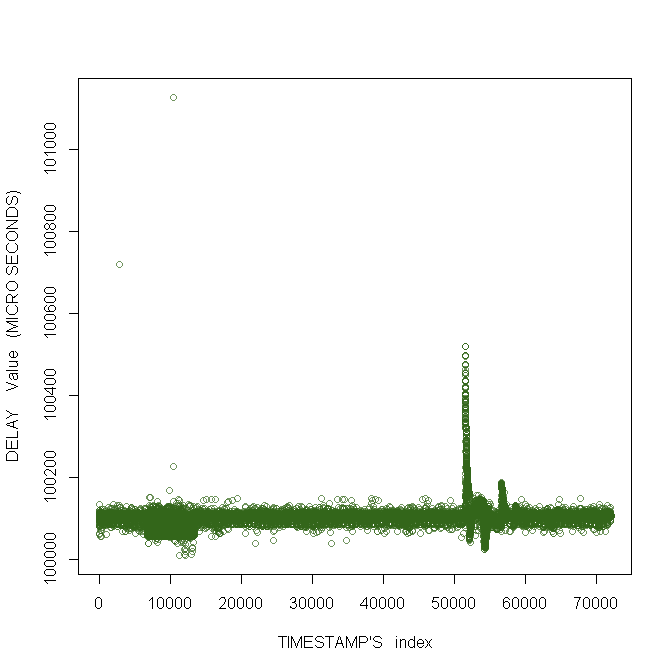
\includegraphics[width=0.5\textwidth]{images/simple.png}
\end{figure}
\begin{figure}[H]
    \caption{\centeringΚατανομή τιμών των διαστημάτων μεσολάβησης μεταξύ 2 δειγματοληψιών του αλγορίθμου \textlatin{simple}}
    \centering
    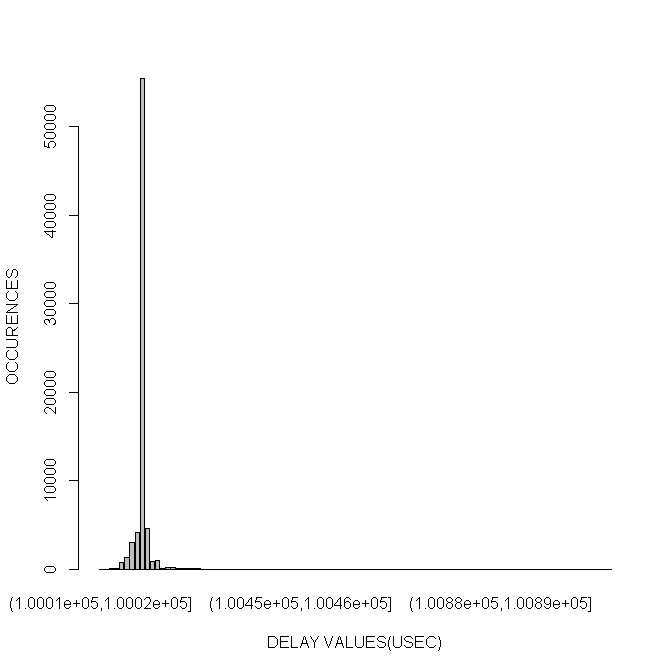
\includegraphics[width=0.5\textwidth]{images/simple_distribution.png}

\end{figure}
\pagebreak



\subsection{Αποτελέσματα αλγορίθμου \textlatin{advanced}.}
\justify
Η εκτέλεση του αλγορίθμου αυτού με ορίσματα:
\begin{itemize}
    \item $executionTime \longleftarrow 2$
    \item $interval \longleftarrow 0.1$
\end{itemize}
είχε συνολικό χρόνο: $7200.000108$ $secs$ δηλαδή καθυστέρησε για περίπου \textbf{0.000108} δευτερόλεπτα ή 108 μικρο-δευτερόλεπτα. Η μέση τιμή ήταν \textbf{100000.0015 \textlatin{usec}}, δηλαδή μεταξύ κάθε κάθε μέτρησης υπήρχε καθυστέρηση περίπου 0.0015 μικρο-δευτερολέπτων. Η τυπική απόκλιση ήταν \textbf{9.14}.
\begin{figure}[h]
\caption{\centering{Τιμές διαστημάτων μεσολάβησης μεταξύ 2 δειγματοληψιών του αλγορίθμου \textlatin{advanced}}}
\centering
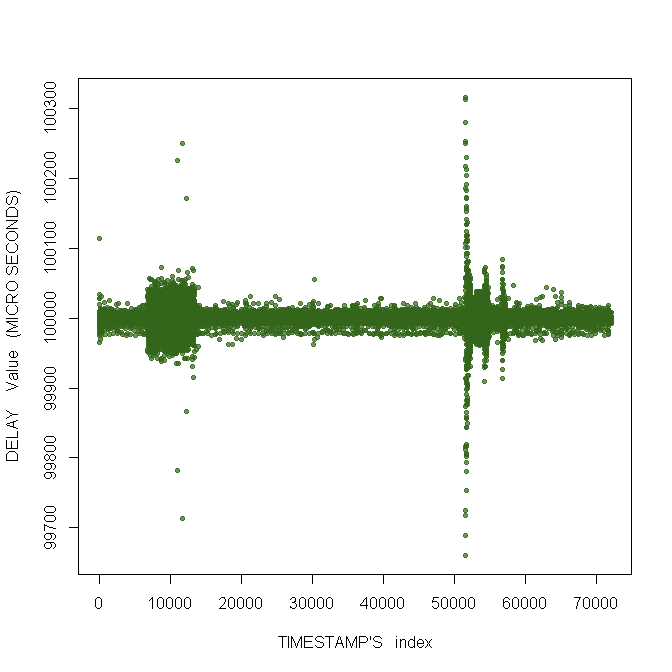
\includegraphics[width=0.5\textwidth]{images/advanced.png}
\end{figure}

\begin{figure}[h]
 \caption{\centeringΚατανομή τιμών των διαστημάτων μεσολάβησης μεταξύ 2 δειγματοληψιών του αλγορίθμου \textlatin{advanced}}
\centering
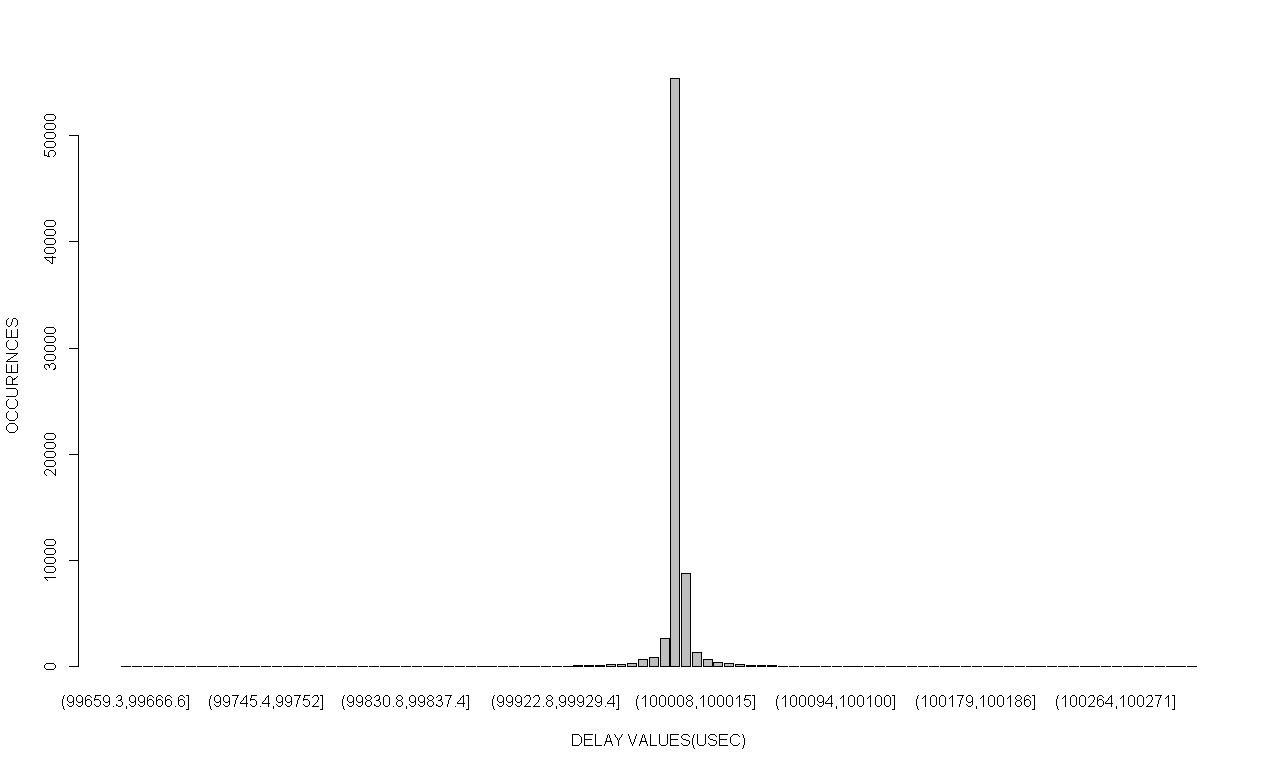
\includegraphics[width=0.5\textwidth]{images/advanced_distribution.png}
\justify
Οπως φαίνεται και από τα παραπάνω διαγράμματα στο σύνολό του οι τιμές κυμάνθηκαν περίπου στα 100000 μικρο-δευτερόλεπτα που ήταν και η επιθυμητή τιμή.
\end{figure}

\newpage

\section{Υπολογιστική ισχύς.}
Κατά την εκτέλεση του πειράματος παρατηρήθηκε και η συμπεριφορά του προγράμματα αναφορικά με την υπολογιστική ισχύ που καταναλώνει.

\justify
Για την παρακολούθηση του προγράμματος κατά τη διάρκεια εκτέλεσης χρησιμοποιήθηκε η εντολή \textlatin{\textbf{top}}.\cite{manual} Τα στοιχεία που ήταν σημαντικά για την παρακολούθηση της διαδικασίας εκτέλεσης ήταν η συγκεκριμένα, για το λόγο αυτό χρησιμοποιήθηκε η ακόλουθη εντολή για την εξαγωγή των αποτελεσμάτων σε μορφή αρχείου ώστε να επεξεργαστούν μετά τα αποτελέσματα κατάλληλα.
\begin{itemize}
    \item \textlatin{\textit{top -b -d 0.01 -p <pid> -n 10000 | awk '/Cpu/||/<user>/ {print}'      > log.txt}}
\end{itemize}
Όπου ύστερα από την παράμετρο \textlatin{\textit{-d}} ακολουθεί το χρονικό διάστημα παρακολούθησης της διεργασίας σε δευτερόλεπτα, \textlatin{\textit{pid}} ο αριθμός της επιθυμητής διεργασίας για παρακολούθηση και \textlatin{\textit{-n}} ο αριθμός των μετρήσεων που θα πραγματοποιήσει η εντολή. Το υπόλοιπο της εντολής χρησιμοποιείται για την εξαγωγή των αποτελεσμάτων σε αρχείο.

\justify 
Η εκτέλεση της παραπάνω εντολής ισοδυναμεί με 10000 μετρήσεις χρονικών διαστημάτων 0.01 δευτερολέπτων. Δηλαδή, αποτελούν ένα ενδεικτικό δείγμα 100 δευτερολέπτων εκτέλεσης. Τα αποτελέσματα αυτά αναλύθηκαν με τη χρήση του \textlatin{script} \textlatin{\textbf{regex.R}} σε γλώσσα \textlatin{\textit{R}}. 
\justify
Στα αποτελέσματα που προέκυψαν η διεργασία αναγνωρίστηκε μόλις \textbf{4} φορές σε κατάσταση \textlatin{\textbf{Running}} και \textbf{9994} φορές σε λειτουργία \textlatin{\textbf{Sleeping}}. 

\justify
Παρατίθενται τα διαγράμματα ποσοστών κατάστασης \textlatin{idle} της διεργασίας ανά μέτρηση, όπως αυτά προέκυψαν από τις παραπάνω μετρήσεις και την ανάλυση. 

\justify
Σημειώνεται για τη μεταβλητή που εξετάζεται ότι αντιπροσωπεύει το ποσοστό χρόνου κατά το οποίο εκτελείται η μέτρηση στο οποίο η διεργασία παραμένει στον \textlatin{kernel idle handler}.\cite{manual}, ή διαφορετικά:
\begin{itemize}
    \item \textlatin{id, idle    : time spent in the kernel idle handler}\cite{manual}
\end{itemize}

\begin{figure}[H]
    \caption{\centering{Τιμές μεταβλητής \textlatin{idle}(\%)}}
    \centering
    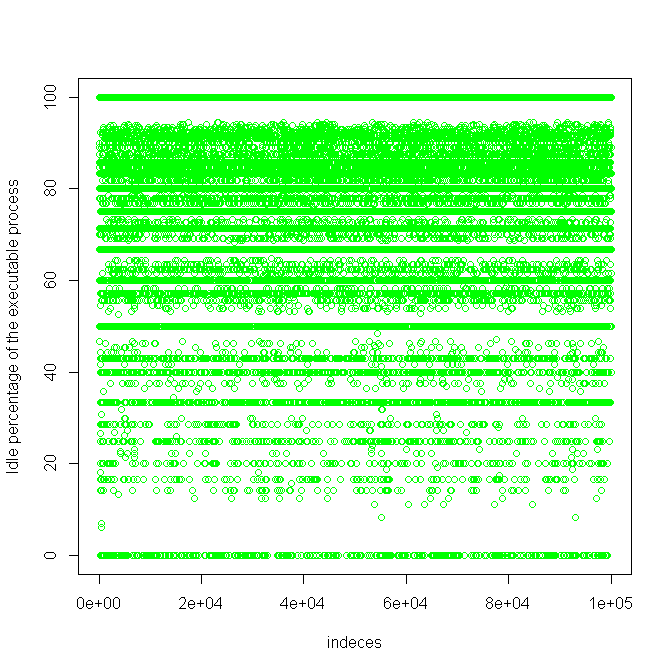
\includegraphics[width=0.5\textwidth]{images/idle.png}
\end{figure}


\begin{figure}[H]
    \caption{\centering{\textlatin{Boxplot} τιμών μεταβλητής \textlatin{idle}(\%)}}
    \centering
    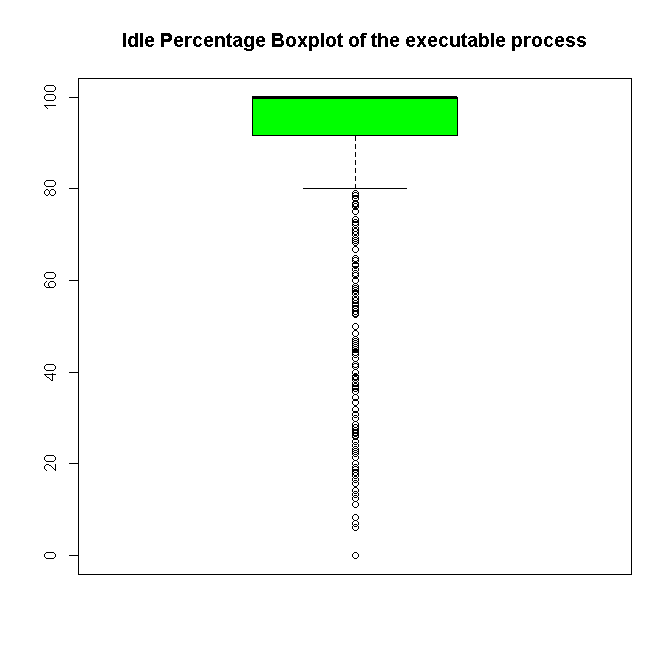
\includegraphics[width=0.5\textwidth]{images/idle_boxpplot.png}
\end{figure}


\section{Συμπεράσματα.}
Τελικά, η εργασία αυτή καταλήγει στο συμπέρασμα ότι η δειγματοληψία τιμών την οποία εκτελεί ένα ενσωματωμένο σύστημα είναι καλό να ελέγχεται και να γίνεται προσπάθεια να είναι όσο το δυνατό ακριβέστερη. Στην παρούσα υλοποίηση παρατηρήθηκε σφάλμα της τάξης του 
\bibliographystyle{plain}
\bibliography{M335}

\end{document}
